% =====================================================================
%  Naive Diversification and the Opportunity Set — LaTeX source
%
%  Formatted to the Portfolio Management Research "Article Submission
%  Guidelines" (Adelson, March 2023), which govern The Journal of
%  Portfolio Management:
%    * 8.5x11, 1 inch margins, 12pt Times New Roman, SINGLE spaced
%    * 12pt space before each paragraph, first line indented
%    * page numbers bottom centre
%    * all tabular and graphical material is an EXHIBIT, numbered in one
%      Arabic sequence in order of appearance ("Do not call them Table 1
%      and Figure 1")
%    * references in Chicago Manual of Style 17th ed. AUTHOR-DATE
%    * first page = title/author only; second = abstract + 3 key
%      takeaways + keywords/JEL; main text begins on the third page
%    * abstract target 160 words, non-technical, NO references
%
%  Build:  pdflatex paper && bibtex-free (bibliography is inline) &&
%          pdflatex paper && pdflatex paper
%  PMR also requires a PDF with all fonts embedded alongside the .tex.
% =====================================================================
\documentclass[12pt,letterpaper]{article}

\usepackage[T1]{fontenc}
\usepackage[utf8]{inputenc}
\usepackage{mathptmx}                 % Times for text and math
\usepackage[margin=1in]{geometry}
\usepackage{graphicx}
\usepackage{amsmath}
\usepackage{booktabs}
\usepackage{float}                    % [H] — keep exhibits where they are written
\usepackage{natbib}
\usepackage[hidelinks]{hyperref}

\graphicspath{{../figures/}}

% Chicago author-date puts NO comma between author and year: "(Smith 2020)".
% natbib's default round style emits "(Smith, 2020)", so the separator is cleared.
\bibpunct{(}{)}{;}{a}{}{,}

% ---- PMR mechanical specs -------------------------------------------
\setlength{\parindent}{0.5in}                 % "indented one tab stop"
\setlength{\parskip}{12pt plus 2pt minus 1pt} % "12 points of space before"
\linespread{1.0}                              % single spaced
\pagestyle{plain}                             % page number, bottom centre

% ---- Exhibits: ONE Arabic sequence across tables and figures ---------
% PMR is explicit that tabular and graphical material share a single
% "Exhibit" series numbered in order of appearance.
% PMR's Appendix A puts the exhibit number and title ABOVE the exhibit (12pt) and the
% source/explanatory note BELOW it (8pt) — for charts as well as tables, which is not the
% usual academic convention of captions under figures. These two macros implement that, and
% owning the counter directly keeps tables and charts in one Arabic sequence.
\newcounter{exhibit}
\renewcommand{\theexhibit}{\arabic{exhibit}}
% Both are used INSIDE a float that has already issued \centering, which sets leftskip,
% rightskip and parfillskip so that every line centres. Undoing those three explicitly is
% what keeps the title flush left and the note justified across the full measure.
\newcommand{\exhibitflush}{%
  \leftskip=0pt\relax \rightskip=0pt\relax
  \parfillskip=0pt plus 1fil\relax \parindent=0pt\relax}
\newcommand{\exhibittitle}[2]{%
  \refstepcounter{exhibit}%
  \par{\exhibitflush\textbf{Exhibit \theexhibit: #1}\label{#2}\par}%
  \vspace{5pt}}
\newcommand{\exhibitnote}[1]{%
  \par\vspace{5pt}%
  {\exhibitflush\fontsize{8}{9.6}\selectfont #1\par}}

% ---- Headings: three levels, PMR style, numbers retained -------------
% PMR specifies bold uppercase / indented bold / bold in-line. It does not
% forbid section numbers, and the text cross-references sections by number
% ("Section 6"), so the numbers are kept.
\makeatletter
\renewcommand{\section}{\@startsection{section}{1}{0pt}%
  {14pt plus 2pt}{6pt}{\normalfont\bfseries\MakeUppercase}}
\renewcommand{\subsection}{\@startsection{subsection}{2}{\parindent}%
  {12pt plus 2pt}{4pt}{\normalfont\bfseries}}
\renewcommand{\subsubsection}{\@startsection{subsubsection}{3}{\parindent}%
  {10pt}{-1em}{\normalfont\bfseries}}
\makeatother

\newcommand{\head}[1]{\noindent\textbf{#1}\hspace{0.5em}\ignorespaces}

\begin{document}

% =====================================================================
%  FIRST PAGE — title, date, author, contact, role sentence
% =====================================================================
\thispagestyle{empty}
\vspace*{1.5in}
\begin{center}
{\large\bfseries Naive Diversification and the Opportunity Set:\\[2pt]
Long-Only Equity Factor Indices}\\[24pt]
August 2026
\end{center}

\vspace{0.6in}
\noindent Pau Notari Mart\'i\\
\indent Independent researcher\\
\indent Valencian Community, Spain\\
\indent pau.notari@gmail.com

\vspace{18pt}
% PMR asks for one sentence giving each author's role and affiliation. With no
% institution behind the work, saying so plainly is the accurate version.
\noindent Pau Notari Mart\'i is a computer engineer based in the Valencian Community,
Spain, and conducted this research independently of any institutional affiliation.

\vspace{18pt}
\noindent\emph{Every number in this article is an entry in the project's
critical-findings ledger (M1--M41), names the module that produces it, and regenerates with one command from the
sources listed in the data availability statement. Repository: [URL on publication].}

\clearpage

% =====================================================================
%  SECOND PAGE — abstract, key takeaways, keywords, JEL
% =====================================================================
\thispagestyle{empty}
\begin{center}
{\large\bfseries Naive Diversification and the Opportunity Set:\\[2pt]
Long-Only Equity Factor Indices}\\[16pt]
August 2026
\end{center}

\vspace{12pt}
\section*{ABSTRACT}

For twenty years the argument over whether portfolio optimization beats simple equal
weighting has run without resolution. We show that it turns on something neither side
measures: the menu of assets on offer.

On the menu a real investor can reach, twenty-eight long-only regional factor indices, no
optimization rule beats equal weighting by a margin this much data can settle. The optimizers
are not at fault. These indices are close to being the same bet. Long-only factor tilts within
a region move almost in lockstep, so twenty-eight of them carry barely more independent risk
than one does, and no weighting scheme can manufacture diversification the menu does not
contain. Three asset classes, Treasuries, gold and cash, add more of it than all twenty-eight
equity indices combined.

Optimization pays where holdings genuinely differ, and an investable factor menu offers very
little difference to exploit. For a retail investor the problem is one of selection rather than
weighting: widen the menu before refining the weights.

\section*{KEY TAKEAWAYS}

\begin{itemize}\setlength{\itemsep}{6pt}\setlength{\parskip}{0pt}
\item On the menu a retail investor can reach, no weighting rule beats equal weight
      by a margin this data can resolve: at 56\% power, a real edge of that size would go
      undetected nearly half the time.
\item The binding constraint is the menu, not the optimizer. Twenty-eight long-only
      \emph{equity} factor indices hold 1.31 independent risk bets, and adding Treasuries,
      gold and cash buys more than all of them.
\item Widen the menu before refining the weights. Optimization pays where holdings
      genuinely differ, and an investable equity factor menu offers very little difference
      to exploit.
\end{itemize}

\vspace{12pt}
\noindent\textbf{Keywords:} portfolio choice; estimation error; naive
diversification; diversification ratio; backtest overfitting; replication.

\noindent\textbf{JEL classification:} G11, C58.

\clearpage

% =====================================================================
%  MAIN TEXT — begins on the third page.
%  PMR: "Articles in PMR publications do not include any heading before
%  an article's introductory material." The introduction therefore carries
%  no heading, and the counter is advanced so the first visible heading is
%  Section 2 — which is what the prose cross-references point at. Nothing
%  in the text refers to "Section 1".
% =====================================================================

Whether portfolio optimization beats naive equal weight is one of the
longest-running unresolved questions in asset allocation, and the disagreement
is unusually sharp. \citet{demiguel2009} found that across fourteen models and
seven datasets nothing consistently beats 1/N out of sample, and the most recent
replication, on the original datasets extended twenty years through the global
financial crisis and the pandemic, reaches the same verdict
\citep{gelmini2024}. An equally serious literature holds that the result is an
artifact. On that account 1/N wins only because the optimizers were fed
short-window sample means \citep{kritzman2010}, or because they were tested in
high-turnover forms that transaction costs destroy \citep{kirby2012}. Both sides
show real out-of-sample evidence. The debate has stayed open because it has been
argued as though it had a single answer.

It does not, and this article locates the answer. Whether optimization beats 1/N
turns on five things: the dispersion of the asset menu, the length and quality of
the estimation inputs, how much turnover the strategy generates, whether short
sales and leverage are permitted, and how demanding a bar ``beat'' must clear.
Fix all five at the position a real retail investor occupies, a \emph{long-only, index-based, factor-tilted equity menu} with realistic data length, transaction
costs charged and statistical significance required, and the question has a clean answer. On that menu no weighting rule beats 1/N at
conventional significance, and Section 5.1 reports the power behind that
statement rather than leaving it implied. The cause is a property of the menu
itself, which holds about one independent bet, leaving no dispersion for any
scheme to exploit. The optimization defenders are right on their datasets, where
dispersion is high. We are right on ours, where it is not. The two findings are
compatible once the opportunity set is named. Section 6 measures it
(Exhibits~\ref{ex:frontier} and~\ref{ex:dispersion}).

We reach it by fielding the canonical construction rules, together with the three
most-cited rules built specifically to beat 1/N, against each other under one
protocol, attaching a $p$-value to every ranking sentence. Our contributions are
three.

\begin{enumerate}\setlength{\itemsep}{6pt}
\item \textbf{The reconciling finding: dispersion, not method.} We measure why
1/N is unbeatable on an investable factor menu. The diversification ratio implies
1.31 independent bets (95\% confidence interval 1.24 to 1.40 by circular block
bootstrap), long-only factor tilts co-move at 0.885, and the covariance is
near-singular. The mechanism is confirmed by contrast: adding three asset classes
raises the ratio to 1.43, a paired difference of $+0.120$ at $p = 0.0002$, and
moves the menu's minimum pairwise correlation from 0.53 to $-0.14$. This places
the twenty-year 1/N debate on a single axis, the opportunity set.

\item \textbf{A fully instrumented adjudication.} We run the following as
standing diagnostics on every build: \citet{ledoit2008} bootstrap Sharpe
inference (the robust successor to the Jobson-Korkie test of \citeyear{jobson1981} that the prior replication uses), deflated Sharpe ratios \citep{bailey2014}, a Friedman-Nemenyi joint test
\citep{demsar2006}, the combinatorially symmetric cross-validation (CSCV) probability of backtest overfitting \citep{bailey2017}, leave-one-region-out re-races, and sensitivity grids over costs, refit cadence,
constraints, block length and the covariance estimator. Under it, all three
published ``beat-1/N'' rules we field fail. \citeauthor{yuan2023}'s
\citeyearpar{yuan2023} combination loses outright, \citeauthor{brodie2009}'s
\citeyearpar{brodie2009} sparse portfolio reaches only $p = 0.149$, and HERC
lands below both its parents.

\item \textbf{Two null results.} We build, freeze and
pre-register a regime-conditioned shrinkage estimator, then attack it, and the
macro regime signal it depends on, with placebo tests on the regime layer. Both return nothing resolvable at this sample size. We report the
negative result with a power post-mortem.
\end{enumerate}

Section 2 places the article in the five-lever debate. Sections 3 and 4 give the
data and the protocol, Section 5 runs the race, and Section 6, the contribution,
measures why it comes out the way it does. Sections 7 and 8 report the nulls and
the robustness checks.

\setcounter{section}{1}
\section{The debate and its five levers}

The two camps rarely engage on the same terms. On one side, \citet{demiguel2009}
and, most recently, \citet{gelmini2024} find 1/N is not systematically beaten out
of sample. On the other, \citet{kritzman2010}, titling their rebuttal ``the
fallacy of 1/N,'' and \citet{kirby2012} show optimization can win. Read together,
their disagreement concerns experimental conditions, and it resolves into five
levers. (i) \emph{Menu dispersion}: DeMiguel's own explanation, quoted approvingly
by Gelmini and Uberti, is that optimization improves relative to 1/N when
idiosyncratic volatility is high and the covariance is far from singular.
(ii) \emph{Estimation inputs}: Kritzman et al.\ locate 1/N's edge in short-window
sample means. Gelmini and Uberti test the lever directly and find a growing window
helps the optimizers without producing a systematic win. (iii) \emph{Turnover}:
Kirby and Ostdiek attribute the result to the extreme turnover of the strategies
DeMiguel tested. (iv) \emph{Short sales and leverage}: much of the measured
optimization advantage requires positions a long-only investor cannot take.
(v) \emph{The significance bar}: pro-optimization evidence is often point-estimate
or single-dataset, whereas the humility side demands significance across datasets.
\citet{pflug2012} supply the theory the humility side otherwise lacks, showing 1/N
optimal under sufficient model ambiguity, which is the regime a retail investor
with a few decades of data inhabits. We fix all five levers at that retail
position.

\head{Estimation error.} \citet{markowitz1952} optimality collides with sampling
error \citep{michaud1989,chopra1993}, which \citet{demiguel2009} quantify.
\citet{yuan2023} supply the missing theory. The plug-in Sharpe converges to
$\tau \cdot SR$ with $\tau = \sqrt{(1-\eta)/(1+\eta/SR^{2})}$ and $\eta = N/T$,
and under a one-factor structure 1/N is asymptotically optimal as $N$ grows. They
then beat 1/N with a closed-form combination of the plug-in global
minimum-variance portfolio and 1/N. We field their rule (Section 5), where it
loses on our menu, an outcome their own Proposition 3 and their $T = 360$ window
requirement predict in advance. The humility result therefore survives its
strongest published challenger, adjudicated with that challenger's mathematics.

\head{Menu selection.} A weighting study is only as interesting as its menu.
\citet{ilmanen2012} report average correlation near zero across \emph{factor}
constituents against roughly 0.4 across asset classes, which is why a
factor-spanning menu should diversify more per slot. We measure our own menu with
the metric that literature standardized, the \citet{choueifaty2008}
diversification ratio, whose square estimates the number of independent risk bets.
Section 6 shows that the long-only wrapper destroys most of the effect.
\citet{hurst2017} point at a diversifier we do not hold. We field the rule form of
trend here and flag the asset form as the more promising route.

\head{Structural weighting rules.} Risk parity and equal risk contribution
\citep{maillard2010,asness2012}, hierarchical risk parity \citep{lopezdeprado2016}
and minimum variance \citep{clarke2006}, whose success the low-volatility anomaly
explains \citep{haugen1991,frazzini2014}, win by imposing structure instead of
estimating means. \citet{antonov2025} supply the theory hierarchical risk parity
lacked, showing analytically that its weights carry less estimation-induced noise
than plug-in Markowitz's. \citet{raffinot2018} hybridizes the two families as
HERC, with a gap-index cluster count after \citet{tibshirani2001}. We field both
linkages, since reporting only the flattering one is how hyperparameters get
hidden.

\head{Constraints, sparsity and shrinkage.} \citet{jagannathan2003} showed weight
constraints act as covariance shrinkage, and we measure the effect prospectively
in Section 5.2. \citet{brodie2009} regularize Markowitz with an $\ell_1$ penalty
and outperform 1/N on 48 industry portfolios, but that penalty is inert without
shorting (Section 4.2), which makes them the selecting sibling of our spreading
constraints and the natural contestant to field with the two things their claim
lacked, a Sharpe-difference test and transaction costs.
\citet{demiguel2009norm} are the norm-constrained cousin. On the input side,
\citet{jorion1986} and \citet{frost1986} shrink means toward within-sample grand
means, whereas ours (Section 4.1) shrinks conditional means toward another era's
evidence under a pretest gate in the \citet{judge1978} lineage.
\citet{boyd2024} show what Markowitz looks like when the inputs are genuinely
there, which is the opposite of the regime we study.

\head{Regime models and inference.} \citet{ang2002,ang2004} established that
regimes matter for allocation, and \citet{guidolin2007} extended the latent-state
machinery. We differ in kind, using an observable deterministic classifier and
pooled sample means, with nothing fitted to predict. For inference we implement,
in code, \citet{ledoit2008}, \citet{bailey2014}, \citet{bailey2017},
\citet{demsar2006} and \citet{politis1994}. \citeauthor{ledoit2020}'s
\citeyearpar{ledoit2020} analytical nonlinear shrinkage enters as a sensitivity
dimension on the covariance estimator every risk number rides on.

\section{Data and the investor's constraint set}

The menu is not an arbitrary choice of dataset. It is a \emph{position}, and the
article's question only means something once that position is stated. We study a
retail investor who is \emph{long-only, unlevered, index-based and long-horizon}, the constraint set of someone buying liquid, low-cost ETFs rather
than running a book. We price the equity-heavy stance without recommending it.
Our scenario cones put an equity profile's probability of cumulative loss at
approximately 14\% at 5 years against a defensive multi-asset profile's 1.4\%,
but at 20 years the two are 1.2\% and 0.0\% with the equity profile's median
compound annual growth rate still materially higher (approximately 9.7\% versus
7.3\%). Converging \emph{loss probability} is not converging \emph{risk}, since
terminal-wealth dispersion grows with horizon, and these are simulations under a
re-sequenced-history assumption, not forecasts.

The factor tilts are justified by documented return premia and not by
diversification: value and size \citep{fama1993}, momentum \citep{jegadeesh1993}
and quality \citep{asness2019}, with \citet{asness2013} supplying the strongest
anti-data-mining defence. We call each index line, one per region and factor, a sleeve; a region's Reference sleeve is its plain market index, carrying no factor tilt. On our own sleeves every
factor beats its regional Reference in compound annual growth over the full window (Enhanced Value
$+3.70$pt, Momentum $+2.88$pt, Quality $+1.47$pt, winning in 7 of 7, 7 of 7 and
6 of 6 regions). Restricted to the backfill-free live-index era (2015 onward) the premia shrink but survive, with
Momentum $+3.38$pt, Enhanced Value $+1.76$pt and Quality $+1.04$pt, the last
winning in only 4 of 6 regions. That attenuation is consistent with
\citeauthor{mclean2016}'s \citeyearpar{mclean2016} post-publication decay, and it
is the magnitude a prospective investor should plan around. Section 6 measures
that in long-only form these tilts do not diversify.

\head{Sources.} The modern menu is 28 MSCI region-by-factor indices (ACWI, World,
World ex-USA, USA, EM, Europe, AC Asia ex-Japan, Japan, crossed with Reference, Momentum, Enhanced Value and Quality), monthly net-USD total returns,
common window January 1999 to June 2026 (330 months). Four of the 32 possible combinations have
no index, which is why the menu is 28 rather than 32: Europe has no Quality sleeve, World none
for Enhanced Value, and World ex-USA neither Momentum nor Quality. The menu is redundant by
construction, with a mean pairwise correlation of 0.76 and a first principal component
explaining 77\% of variance.

Two summaries of that redundancy recur below and answer different questions, so we distinguish
them once here. The eigenvalue-entropy effective bet count (approximately 2.8) measures how
many components the variance is spread over. The Choueifaty-Coignard $DR^{2}$ (1.31, Section 6)
measures how much of the sleeves' standalone risk the correlations actually cancel under the
weights held. A menu can spread variance over several components while cancelling almost none
of it, which is exactly this menu. All headline statements use $DR^{2}$.

Sixteen FRED indicators feed a four-quadrant growth-by-inflation classifier, used
for descriptive statistics only with no fitted latent-state model. For long
history we use Ken French research factors (1926 onward) and six long-only
size-by-value portfolios, 10-year US Treasury total returns constructed from the
FRED yield by the \citet{swinkels2019} par-bond approximation (sanity check: 2008
$+21$\%, 2022 $-16$\%), LBMA gold and Treasury bill returns. These are research
constructs and never investable sleeves. The classifier labels months from 1960
(789 months, 2.4 times the modern window, containing the actual 1970s
stagflation). Finally, a \emph{virgin confirmatory universe}: nine Ken French
international sleeves (Europe, Japan and Asia-Pacific ex-Japan, crossed with
market, value and momentum), USD, monthly, from November 1990 onward, never
downloaded or inspected during development, with the test protocol and thresholds
committed to the repository before the single run (Section 8).

\section{Method}

\subsection{The regime layer and a pre-registered estimator}

Growth and inflation composites (z-scored, sign-adjusted trends of several
indicators each) define four quadrants: Goldilocks, Reflation, Deflationary bust
and Stagflation, with soft probabilities and an empirical monthly transition
matrix. Two design facts matter downstream. The classifier is deterministic and
identical across eras, and its per-quadrant factor patterns are structural, with
15 of 16 factor-by-quadrant sign cells agreeing between 1960--2026 and the modern
window. The single flip is the market factor in stagflation.

On top of it we build, freeze and pre-register a transparent estimator for the
noisiest objects in the exercise, the per-regime conditional means, at 30 to 90
monthly observations per cell. We state it because Section 7.2 reports that it has
no effect resolvable at this sample size, and the construction and its
null result are inseparable. Write $\hat{e}_{is}$ for the modern conditional excess of factor sleeve $i$ in state $s$:
the mean monthly return of $i$ across the training months labelled $s$, minus the mean of its
regional Reference sleeve across the same months. Each factor family maps to a long counterpart
$j$ among the Fama-French research factors, Enhanced Value to HML and Momentum to MOM, with
Quality having none and staying modern. Then $\bar{f}_{js}$ is that counterpart's mean return in
state $s$ over the 66-year sample and $\bar{f}^{\,\prime}_{js}$ is the same quantity over the
modern window alone. The two sample sizes are the months available in state $s$ on each side,
$n_s$ modern and $m_s$ long, and $m_s \gg n_s$ throughout: 789 classifiable long months against
roughly 330 modern ones, which is why the anchor dominates wherever the gate opens. Finally
$\beta_j$ translates academic long-short factor units into long-only sleeve excess units,
estimated once per family as the ordinary-least-squares slope of the pooled modern sleeve excess
on $f_j$ over their overlap; measured values run from 0.19 to 0.28. With $\mathbf{1}\{\cdot\}$
the indicator function, the estimator is a gate and a blend

\begin{equation}
g_{js} = \mathbf{1}\!\left\{ \operatorname{sign}(\bar{f}_{js})
       = \operatorname{sign}(\bar{f}^{\,\prime}_{js}) \right\}
\end{equation}

\begin{equation}
\tilde{e}_{is} = g_{js} \cdot
  \frac{n_s \hat{e}_{is} + m_s \beta_j \bar{f}_{js}}{n_s + m_s}
  + (1 - g_{js})\, \hat{e}_{is}
\end{equation}

The gate asks one question of the long series: does its 66-year record in state $s$ agree in
sign with what that same series did in the modern era? If the two eras disagree about direction,
nothing transfers and the modern estimate stands. If they agree, the blend is a precision-weighted
average of the modern estimate and the $\beta$-mapped long one, weighted by the months of evidence
behind each. This is empirical-Bayes pooling with a pretest gate on the crudest sufficient
statistic, the sign. It feeds the
\citet{black1992} view vector and the worst-quadrant objective's per-regime means,
and reporting always shows raw modern means. Full treatment, including the
asset-class and no-counterpart cases, is in the repository.

\subsection{Contestants, protocol and inference}

We field equal weight (1/N), minimum variance, equal risk contribution and
hierarchical risk parity (all on \citet{ledoit2004} shrunk covariances), a mean-variance blend built around a Black-Litterman posterior, which the exhibits label the Black-Litterman blend,
cross-sectional momentum (12-1, top 6), unlevered volatility targeting
\citep{moreira2017}, binary trend overlays \citep{faber2007,antonacci2014},
worst-quadrant maximin, which maximizes the mean return in whichever of the four macro states turns out worst, both unconstrained and under diversified caps (per-sleeve at most 25\%, look-through geographic at most 40\%, factor at most 40\%), and an
all-weather diversified maximin on the menu extended with Treasury, gold and cash
proxies. We also field the three most-cited ``beat-1/N'' rules as contestants: the
\citet{yuan2023} global minimum-variance combination, the \citet{brodie2009}
sparse portfolio (in long-only form minimum variance at a target return, the
$\ell_1$ penalty being inert), and HERC in both linkages. Raw full-sample mean
returns are forbidden as objective inputs throughout.

The protocol is an expanding-window walk-forward with a 120-month warmup, annual
refits, every input re-estimated on training data only, and returns net of 10
basis points of one-way transaction costs on turnover. Companion races are a
90-year re-race on the proxy universe (out of sample 1936--2026) with
shifted-start variants, hand-dated episode replays, and a regime-persistent
stationary bootstrap used as forward validator and never as objective. Inference
is \citet{ledoit2008} heteroskedasticity- and autocorrelation-consistent
delta-method plus a studentized circular block bootstrap ($B = 4999$,
$b \approx T^{1/3}$, sensitivity $b \in \{3,6,10\}$) for every contestant against 1/N and against minimum variance as the incumbent winner, deflated Sharpe with the fielded-roster
trial count, and CSCV probability of backtest overfitting ($S = 16$, 12,870
half-splits). We use the bootstrap rather than the classical Sharpe test because
monthly Sharpe differences carry heavy tails and autocorrelation, which that test
assumes away.

Sharpe ratios use a zero risk-free rate throughout, tables and text alike. On the
148 of 210 out-of-sample months for which a Treasury-bill series is available,
recomputing in excess terms on that same subset moves the headline $p$ from 0.180
to 0.209 and the Sharpe gap from $+0.163$ to $+0.151$, so the convention is not
load-bearing. What separates those figures from the 0.055 of the full sample is
the shorter window, not the choice of convention.

\section{The walk-forward race}

\subsection{The modern menu, 2009--2026}

\begin{table}[H]
\centering
\exhibittitle{Walk-forward out-of-sample results, 2009--2026}{ex:race}
\fontsize{9}{11}\selectfont
\begin{tabular}{lrrrrrrr}
\toprule
Contestant & CAGR & Vol & Sharpe & maxDD & $\Delta$ Sharpe & $p$ vs 1/N & DSR \\
\midrule
Min-variance                  & 13.8\% & 13.5\% & 1.03 & $-28$\% & $+0.20$ & 0.055 & 1.00 \\
Min-variance + vol-target     & 10.9\% & 11.9\% & 0.94 & $-24$\% & $+0.11$ & 0.304 & 1.00 \\
Sparse Markowitz (Brodie)     & 12.6\% & 13.8\% & 0.93 & $-26$\% & $+0.10$ & 0.149 & 1.00 \\
Maximin (all-weather div.)    &  8.0\% &  8.7\% & 0.93 & $-18$\% & $+0.10$ & 0.611 & 1.00 \\
Hierarchical risk parity      & 12.4\% & 14.8\% & 0.87 & $-27$\% & $+0.04$ & 0.142 & 0.99 \\
Equal risk contribution       & 12.2\% & 15.0\% & 0.85 & $-27$\% & $+0.02$ & 0.191 & 0.99 \\
Maximin (diversified)         & 13.1\% & 16.3\% & 0.84 & $-28$\% & $+0.01$ & 0.839 & 0.99 \\
\textbf{1/N}                  & 12.2\% & 15.3\% & 0.83 & $-27$\% & ---     & ---   & 0.99 \\
HERC (Ward linkage)           & 11.5\% & 15.0\% & 0.80 & $-28$\% & $-0.03$ & 0.573 & 0.99 \\
HERC (single linkage)         & 10.7\% & 14.1\% & 0.80 & $-27$\% & $-0.03$ & 0.576 & 0.99 \\
GMV combination (Yuan-Zhou)   &  9.8\% & 14.2\% & 0.74 & $-30$\% & $-0.10$ & 0.449 & 0.98 \\
Momentum 12-1 (top 6)         & 10.8\% & 16.0\% & 0.72 & $-29$\% & $-0.11$ & 0.235 & 0.97 \\
Maximin (worst quadrant)      & 12.4\% & 18.9\% & 0.71 & $-28$\% & $-0.12$ & 0.235 & 0.98 \\
Black-Litterman blend & 11.2\% & 17.3\% & 0.70 & $-27$\% & $-0.13$ & 0.070 & 0.97 \\
1/N + vol-target              &  8.5\% & 12.9\% & 0.70 & $-26$\% & $-0.13$ & \textbf{0.009} & 0.96 \\
1/N + trend (10m SMA)         &  6.8\% & 11.0\% & 0.66 & $-20$\% & $-0.17$ & 0.326 & 0.95 \\
Dual momentum                 &  5.4\% & 13.3\% & 0.46 & $-27$\% & $-0.37$ & \textbf{0.034} & 0.81 \\
\bottomrule
\end{tabular}
\exhibitnote{210 out-of-sample months, net of 10 basis points of transaction
costs. $\Delta$ Sharpe and $p$ (studentized circular block bootstrap,
\citealp{ledoit2008}) are against 1/N. DSR is the deflated Sharpe ratio against
the fielded roster. Sorted by Sharpe ratio.}
\end{table}

Exhibit~\ref{ex:race} has one headline. Minimum variance tops it, and its edge over 1/N is
not significant.

The rest of the table says the same thing in different ways. No contestant clears 5\% against
equal weight: minimum variance reaches a bootstrap $p$ of 0.055 and every other rule sits at
$p \ge 0.14$. What the data can detect is the downside. Equal weight plus volatility targeting
is significantly worse than plain 1/N, and dual momentum worse still.

The verdict survives a joint test as well as the pairwise ones. A Friedman test on 12-month
block ranks rejects the null that the ordering is noise ($\chi^{2} = 46.6$), yet the Nemenyi
critical difference clears no contestant past 1/N. The ranking is real; the gap to equal weight
is not. Multiplicity does not rescue anything either: deflated Sharpe ratios of 0.98 and above
clear that bar, and the probability that the in-sample-selected contestant is no better than
the out-of-sample median is 33\%, which is real selection information well short of
certainty.

\head{What that non-rejection is worth.} A $p$ above 0.05 licenses ``no effect''
only if the design could have found one, so we report the power of our own
headline test, meaning the chance it would have flagged an edge of that size as
significant had one really existed, computed on the same standard error the test
uses. Against the largest gap
in Exhibit~\ref{ex:race}, minimum variance's $+0.20$ annualized Sharpe, the design
has 56\% power at the 5\% level. The smallest gap the design could detect at a given target power, its minimum detectable effect size, follows from the same standard error. Writing $\pi$ for that target and $\alpha$ for the significance level,

\begin{equation}
\mathrm{MDES} \;=\; \left(z_{1-\alpha/2} + z_{\pi}\right) \mathrm{se},
\end{equation}

\noindent where $z$ denotes a standard normal quantile. At $\alpha = 0.05$ and $\pi = 0.80$ the
bracket is 2.80, so the minimum detectable gap is 2.80 standard errors, or $+0.27$
annualized Sharpe here. Because $\mathrm{se}$ falls with $\sqrt{T}$, that
threshold is a property of the sample length before it is a property of any estimator. The observed gap is three quarters of the
detectable one. The correct statement is therefore weaker than the literature's
usual phrasing, and we adopt it throughout: no rule beats 1/N resolvably at this sample size. Whether a $+0.20$ edge exists is a question 210 monthly
observations cannot answer either way. Section 6 matters because the menu
measurement is not subject to the same limit.

Two further facts constrain how far the modern race travels, and they point the
same way. The winner's return is 82\% attributable to Quality sleeves (below),
and Quality is the defensive factor a post-2009 window rewards. In the 90-year
proxy race of Section 5.2 the same rule falls to last among structural rules and
beats 1/N in only 25\% of shifted-start windows. The most economical reading of
the two together is that minimum variance's modern lead is a regime-shaped factor
bet and not a durable property of the method.



\begin{figure}[H]
\exhibittitle{No rule clears significance against 1/N, and two overlays are significantly worse}{ex:inference}
\centering
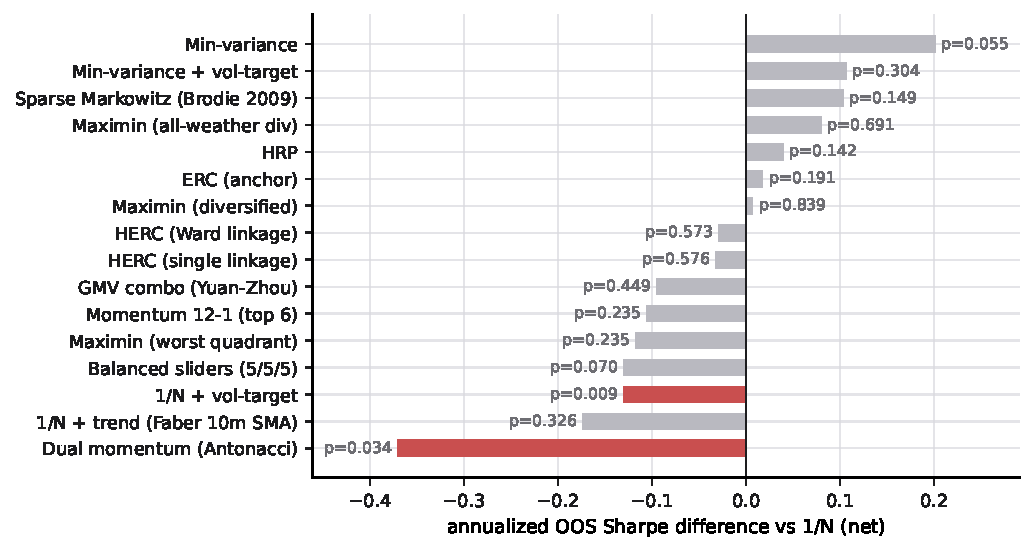
\includegraphics[width=\textwidth]{F2_inference_vs_1N.pdf}
\exhibitnote{Annualized Sharpe difference against 1/N for every contestant, with the
Ledoit-Wolf bootstrap $p$-value on each bar. The two red bars are the overlays that lose
significantly.}
\end{figure}

None of the three most-cited rules designed to beat 1/N does so on this menu. The
\citet{yuan2023} combination loses outright (0.74 against 0.83, $p = 0.45$), which
their own theory predicts where the estimation window is short and the menu
one-factor-dominated, and we declared the prediction before running.
\citeauthor{brodie2009}'s \citeyearpar{brodie2009} sparse portfolio reaches third
place (0.93) at only $p = 0.149$, so their ``significantly and consistently'' does
not survive the Sharpe-difference test and the transaction charge they never
applied. HERC lands below both its parents.

Two mechanical facts explain why nothing separates. The contestants' out-of-sample
returns are 0.93 to 0.998 correlated with one another. Hierarchical risk parity
and equal risk contribution at 0.998 are one portfolio under two names, and
Brodie and minimum variance at 0.975 earn from the same USA Quality sleeve, so
the seventeen-row table is roughly four distinct strategies, and no Sharpe test
can pull apart series that move together this closely. Attribution then shows
what the winner actually is. Minimum variance earns 82\% of its out-of-sample return in Quality sleeves (USA 52\%, World 30\%), which is the
low-volatility-anomaly mechanism made visible: a defensive factor bet carrying an
optimizer's name. Both facts point past the optimizer to the menu, which
Section 6 measures.

\subsection{Long history and the constraint grids}

Re-raced over 1936--2026 on six long-only Fama-French portfolios, minimum variance
falls to last among structural rules (0.71) while hierarchical risk parity (0.76)
and equal risk contribution (0.75) edge 1/N (0.74). Across shifted-start variants
both beat 1/N in 100\% of windows and minimum variance in 25\%. The
modern menu shows the same signature in rolling windows, with equal risk
contribution and hierarchical risk parity beating 1/N in 98 to 99\% of rolling
three-year windows. Structure is the property that travels, and the modern winner
does not.

\begin{figure}[H]
\exhibittitle{No ranking flips in any sensitivity cell}{ex:grids}
\centering
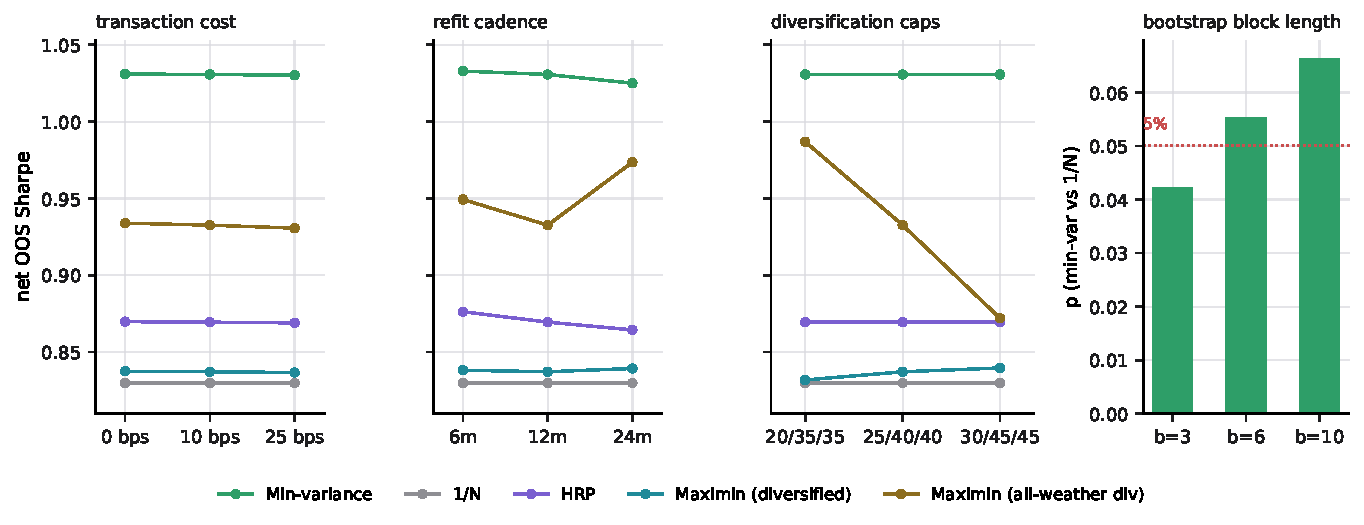
\includegraphics[width=\textwidth]{F5_sensitivity_grids.pdf}
\exhibitnote{Each grid dimension on its own axis, sharing one Sharpe scale. Costs and refit
cadence are flat for every contestant. The one line that moves is the all-weather maximin
under looser caps, from 0.99 down to 0.87, which is constraints-as-shrinkage rather than a
ranking flip. Rightmost panel: the one specification choice that does move the headline $p$-value, the bootstrap block length.}
\end{figure}

Constraints behave as \citet{jagannathan2003} predicted, measured prospectively
rather than in-sample. The capped maximin beats its unconstrained twin out of
sample in every sensitivity-grid cell, by $+0.115$ to $+0.132$ Sharpe across
costs of 0, 10 and 25 basis points, refits of 6, 12 and 24 months, and cap levels
from 20/35/35 through 45/45. No grid cell flips any ranking conclusion. The single
genuine frontier is the headline $p$-value's block-length sensitivity (0.042,
0.055, 0.066). We report the range and do not choose a block length.

\section{The opportunity set}

\begin{figure}[H]
\exhibittitle{The equity menu cannot reach below 13.3\% volatility; the extended menu reaches 0.6\%}{ex:frontier}
\centering
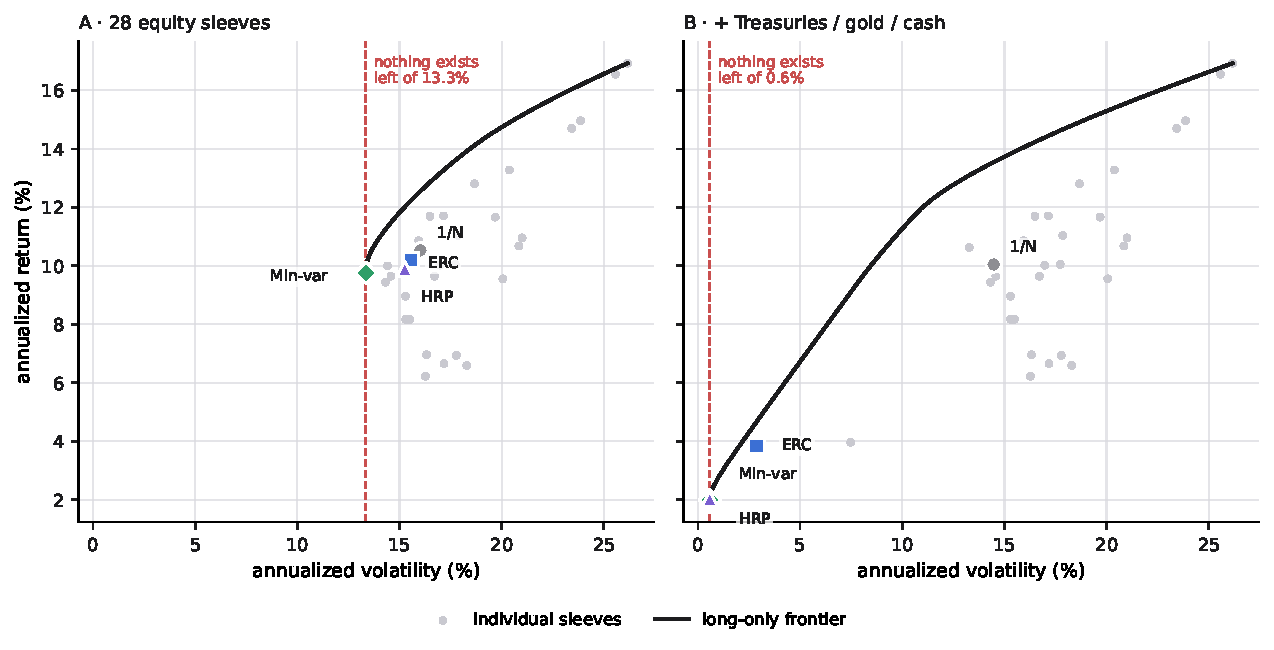
\includegraphics[width=\textwidth]{F0b_frontier_cloud.pdf}
\exhibitnote{The long-only frontier of each menu, with the individual sleeves and the fielded
rules, on a shared scale. Panel A: on 28 equity sleeves the frontier is a short arc and every
rule piles into the same corner. Panel B: adding Treasuries, gold and cash moves the floor to
0.6\% and the frontier sweeps the whole plane. Full-sample geometry, illustrative; the frontier
is solved per target return under long-only weights.}
\end{figure}

Why does no weighting rule beat 1/N here, when the literature's optimization
defenders show that it can? Because on an investable long-only factor menu there
is almost nothing to optimize. We measure it three ways.

\begin{figure}[H]
\exhibittitle{Factor tilts do not decorrelate, and the menu holds about one bet}{ex:dispersion}
\centering
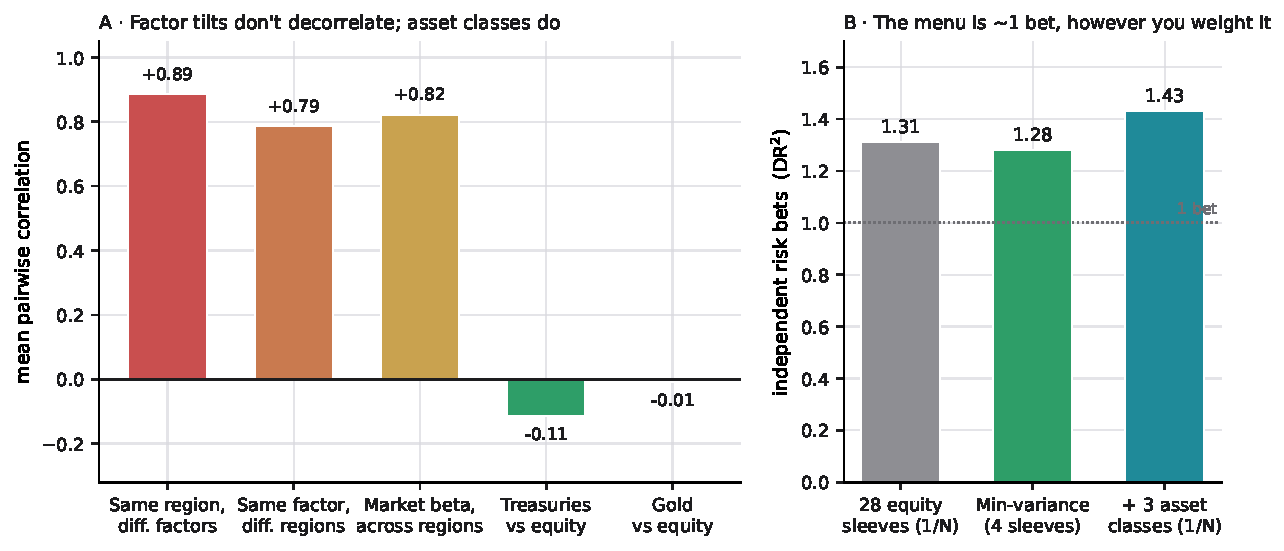
\includegraphics[width=\textwidth]{F0_dispersion.pdf}
\exhibitnote{Grey marks equity-against-equity comparisons throughout the exhibit and teal
marks asset classes. Panel A: the most correlated cut of the menu is same-region,
different-factors (0.885), and only the non-equity sleeves are genuinely different bets
(Treasuries $-0.115$, gold $-0.007$). Panel B: independent risk bets ($DR^{2}$). The shaded band below 1.0 is the
region where a menu holds a single bet, so only the part above it is diversification at all.
The error bar is the 95\% bootstrap interval reported in Section 6.}
\end{figure}

\head{First, correlation structure.} The highest-correlated cut of the entire
menu is \emph{same region, different factors}. Value, momentum and quality within
one country co-move at 0.885, higher than the same factor across regions (0.786)
or pure market beta across regions (0.821). Long-only factor tilts do not
decorrelate, because each index is roughly its parent market plus a small tilt,
and the market beta dominates. The three non-equity proxies are the only genuinely
different bets on the menu, with Treasuries correlating $-0.115$ with the 28
equity sleeves and gold $-0.007$.

\head{Second, independent bets.} The Choueifaty-Coignard diversification ratio compares the
risk of the sleeves held separately with the risk of the portfolio that holds them,

\begin{equation}
DR(w) \;=\; \frac{\sum_i w_i \sigma_i}{\sqrt{w' \Sigma w}},
\end{equation}

\noindent with $\sigma_i$ the standalone volatility of sleeve $i$ and $\Sigma$ the shrunk
covariance. The numerator is what the portfolio's risk would be if the sleeves never offset each
other; the denominator is what it actually is. When correlations cancel nothing the two coincide
and $DR = 1$, which is why $DR^{2}$ reads as an effective number of independent risk bets: it is
1 for a single bet and $N$ for $N$ uncorrelated ones of equal risk. (Defined with $|w_i|$ in
general; every portfolio here is long-only, so $w \ge 0$.) That number is 1.31 for the
equal-weighted equity menu, with a 95\% confidence interval of 1.24 to 1.40. The menu
holds about one and a third independent bets, and that figure is tightly estimated.

We attach inference to it because a contribution reported as a bare point estimate would not be
held to the standard this article applies to every Sharpe comparison. The interval comes from
the block bootstrap of Section 4.2, with the covariance re-shrunk inside every replicate so
that what is measured is the variability of the whole estimate-then-summarize chain rather than
of a fixed covariance.

One objection has to be met before those numbers mean anything. The regional menu nests:
ACWI contains World, which contains the USA, Europe and Japan sleeves, and World ex-USA
contains Europe and Japan. A reader may reasonably ask whether the redundancy is an artefact of
holding the same stocks several times over. It is not. Restricting the calculation to the five
regions that do not overlap, USA, Europe, Japan, emerging markets and AC Asia ex-Japan, leaves
19 sleeves and a $DR^{2}$ of \textbf{1.37} (95\% interval 1.28 to 1.47), slightly higher than
the full menu's 1.31 rather than lower, and the within-region cross-factor correlation is
unchanged at 0.884. Dropping the nested aggregates does not rescue the menu.

Two comparisons put the number in context. The four-sleeve minimum-variance portfolio holds
1.28 independent bets, so the engine whose entire job is to exploit correlations to
cancel risk, holding a quarter as many sleeves, finds no more of them than naive diversification
does. And twenty-four extra equity sleeves buy 0.03 of a bet. The eigenvalues say the same thing: the first principal component alone explains
77\% of variance and the covariance matrix is near-singular.

\head{Third, the contrast that identifies the mechanism.} Adding the three
asset-class proxies moves the menu's minimum pairwise correlation from 0.53 to
$-0.14$ and its diversification ratio to 1.43. Under the paired version of the
same bootstrap, where one set of resampled months drives both menus, the
difference is $+0.120$, with a 95\% interval of $+0.101$ to $+0.144$ and $p = 0.0002$. Three sleeves buy more independent-bet content than twenty-eight
equity sleeves did, and that gap is resolved with a confidence the weighting race
never reaches. At this data scale the menu effect is measurable and the method effect is not.

\subsection{The long-only wrapper}

The literature that motivates factor investing measures \emph{long-short}
portfolios, in which buying the favoured stocks and shorting their opposites
removes the market beta and leaves the premium. An investor who cannot short holds
the premium together with the parent market, and the beta dominates whatever the
tilt contributes. We measure the consequence three independent ways, and they
agree. \emph{(i) Across factors:} \citet{ilmanen2012} report near-zero correlation
across factor constituents, whereas on long-only sleeves the within-region
cross-factor correlation is 0.885, the highest cut of our menu.
\emph{(ii) The value/momentum hedge reverses sign.} \citet{asness2013} put the correlation between the two long-short
premia at approximately $-0.50$, which is the standard argument for
holding both. On our sleeves it is $-0.088$ once each is measured in
excess of its parent index, about a fifth of theirs, and $+0.820$ in the
space an investor actually holds. The direction survives in excess space, so the
economic mechanism is real. The magnitude does not, and in investable form the
sign flips: an investor buying value and momentum indices for their mutual hedge
is buying two versions of the same market exposure. Regional spread is wide and
worth reporting, with Europe ($-0.301$) and Japan ($-0.217$) approaching the
published figure while emerging markets ($+0.017$) and AC Asia ($+0.069$) are
indistinguishable from zero. \emph{(iii) The defensive factor:} Quality's excess
over junk is positive in drawdowns in long-short form, but long-only Quality
carries a beta of 0.91 and \emph{falls in 6 of 6 regions} during the
worst decile of market months, cushioning 0.91 percentage points
($-7.95$\% against the Reference's $-8.87$\%). A cushion of that size is
attenuation and cannot serve as a hedge.

Beta dominance is the mechanism the headline result rests on, and it is why the
diversification the factor literature promises is largely unavailable in the form
a retail investor can buy.

\subsection{The reconciliation}

Optimization beats 1/N exactly where there is dispersion to exploit, on the
industry and factor-portfolio datasets of its defenders, where idiosyncratic
volatility is high and the covariance is well conditioned, which is Gelmini and
Uberti's own explanation (Section 2). An investable factor menu is the opposite
regime, with one dominant bet, a near-singular covariance, and no dispersion for
any weighting scheme to convert into an edge. The disagreement in the literature
concerns the opportunity set, and the retail factor investor sits squarely in the
region where 1/N cannot be beaten.

The practical corollary concerns selection: \emph{widen the menu before refining the weights.} Three asset classes buy more independent-bet content than
twenty-eight equity sleeves, and no amount of estimator sophistication
substitutes.

\section{The extended menu and two null results}

\subsection{A worst-case objective over a regime-diverse menu}

The one construction that measurably changes the risk profile does so through the
menu rather than through regime information. Within equities alone the stagflation
floor was a concentrated Value bet, and forcing diversification collapses it
($+0.31$ to $+0.02$\% per month). Extending the menu with Treasuries and gold
restores the floor at half the volatility, with century-scale shape evidence
behind it: a static all-weather archetype returned $+9.8$\% through the 1973--74
oil shock while a 60/40 portfolio lost 28.5\%. As a walk-forward contestant the
resulting flagship, a capped worst-quadrant portfolio over equities, Treasuries
and gold, delivers a Sharpe ratio of 0.95 at 8.7\% volatility with a $-16.7$\% maximum drawdown, is statistically indistinguishable from minimum variance, the modern winner, at $p = 0.70$ and two thirds of its volatility, and holds the
lowest drawdown in Exhibit~\ref{ex:race}.

Those numbers stand. Their explanation does not. The worst-quadrant objective maximizes the
mean of the worst of four macro partitions of history,

\begin{equation}
\max_{w \in \mathcal{C}} \; \min_{s \in S} \; \mu_s' w,
\end{equation}

\noindent with $\mathcal{C}$ the capped long-only weight set and $\mu_s$ the mean vector in state
$s$. Written this way the problem is visibly a robustness device even when the partitions are
meaningless: the states enter only through the $\mu_s$, so any four-way split of history leaves
the same structure. A capped worst-case allocation over a menu containing genuinely
negatively correlated assets is pushed toward those assets under any four-way
partition, because they are what a worst-case floor rewards. The flagship's record
belongs to the regime-diverse menu and not to knowledge of the regime. The
practical statement survives fully: to buy a shallow-drawdown floor at this data
scale, change what you hold rather than how you time it.

\subsection{Placebo tests of the regime layer}

\begin{figure}[H]
\exhibittitle{Real regime labels land inside the scrambled-label distribution}{ex:placebo}
\centering
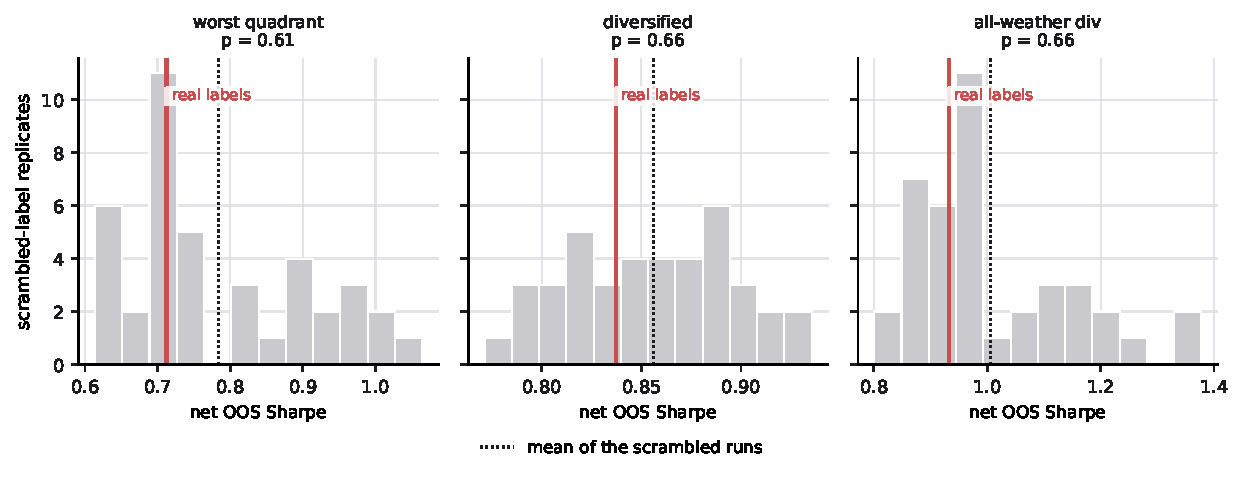
\includegraphics[width=\textwidth]{F7_placebo_null.pdf}
\exhibitnote{Permutation test on the macro-state labels. Grey: net out-of-sample
Sharpe ratio across 40 replicates with the macro-state labels scrambled by a circular rotation,
which preserves run lengths and the transition matrix exactly. Dotted line: the mean of those
scrambled runs. Red line: the real-label result.}
\end{figure}

The regime layer carries the most weight and the least direct evidence, so we test it two ways. \head{The labels.} Re-running the
entire walk-forward 80 times with the macro-state labels scrambled, a circular
rotation preserving marginal frequencies, run lengths and the transition matrix
exactly while destroying only the alignment between a month's label and its
returns, the maximin family performs no better with real labels than with random
ones. On both metrics, net Sharpe ratio and the realized worst-real-quadrant floor
the objective actually optimizes, across twelve cells, the best permutation $p$ is
0.195 and the real labels sit below the scrambled mean in seven of twelve. The
average randomly labelled flagship achieved a better worst-quadrant floor than the
real one. Equal weight, which consumes no labels, is bit-identical across all 81
runs, which serves as a leak check. \head{The estimator.} A paired
difference-of-differences, switching the anchor off and on within each replicate
on the same labels, finds every real-arm effect under half a null standard
deviation and the estimator helping in 45 to 60\% of replicates, a coin flip.

The classifier's descriptive value, meaning
which quadrant we occupy and how factors have behaved per state, is a different
claim and is not tested here. What the placebos settle is narrow. The macro signal does not earn its place in the allocation, and what remains is the negative result together with the apparatus that produced it.

\section{Robustness}

\begin{figure}[H]
\exhibittitle{Only the maximin family changes rank when a region is dropped}{ex:loro}
\centering
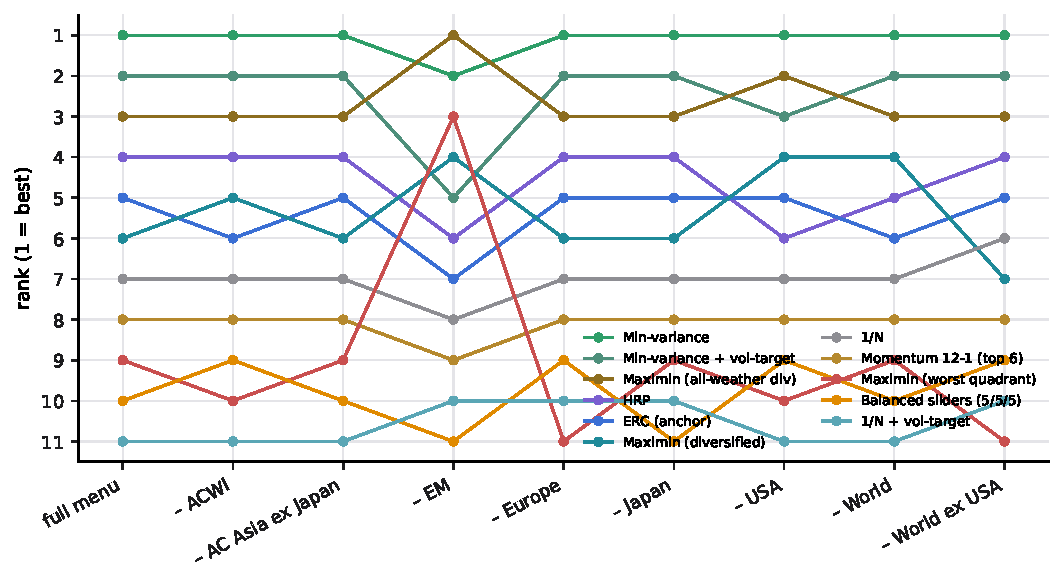
\includegraphics[width=\textwidth]{F3_leave_one_region_out.pdf}
\exhibitnote{Rank of each contestant when a whole region is dropped. Grey lines are every rule
that holds its rank across all nine menus. The worst-quadrant maximin swings eight ranks, and
the all-weather variant takes first place once emerging markets are removed.}
\end{figure}

\head{Exposure and region dependence.} Sub-period splits and region correlations
expose the equity-only maximin as 1/N-like before 2024, correlated 0.93 with
emerging markets and lifted by the 2024-onward rally. The leave-one-region-out
re-race then inverts the naive story. Dropping emerging markets improves every
maximin variant (all-weather 0.93 to 1.18, taking first place), so that exposure
was a net drag the objective was systematically attracted into. The podium itself
is stable across menus. Minimum variance is first in 8 of 9 menus, the all-weather
never leaves the podium, and no overlay beats 1/N on any menu.

\head{Real time and the live era.} Lagging regime labels two months, which is the
realistic macro-publication constraint, improves every regime-dependent contestant
(all-weather 0.93 to 1.11 at 6.6\% volatility), so the shipped results carry no
look-ahead subsidy. Restricting scoring to the live-index era (2015 onward, 138
months) preserves the hierarchy, which answers the pre-launch-backfill critique
with measurement.

\begin{figure}[H]
\exhibittitle{The pre-registered estimator changes nothing on the virgin universe}{ex:virgin}
\centering
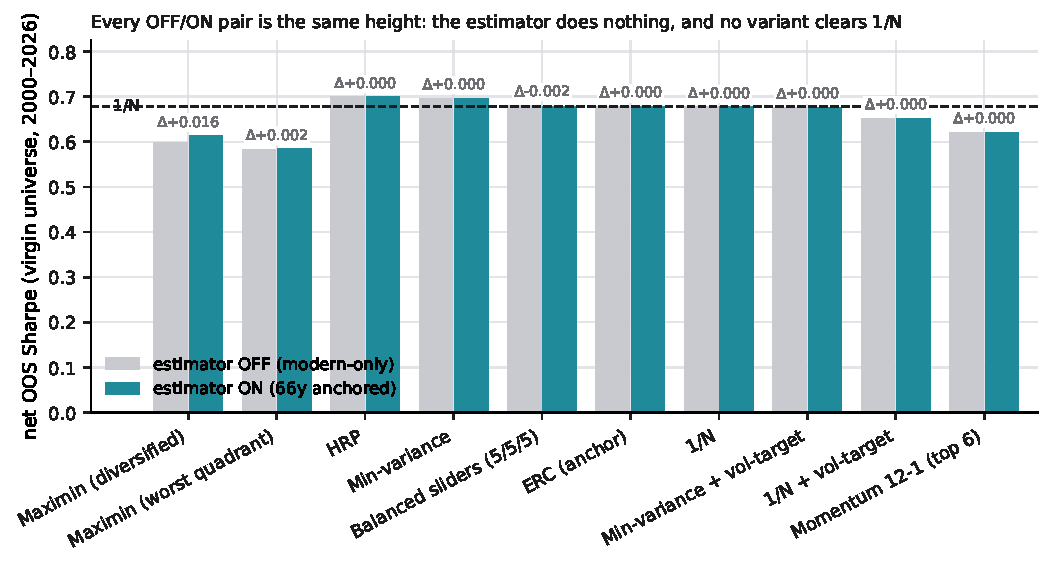
\includegraphics[width=\textwidth]{F4_virgin_universe_ab.pdf}
\exhibitnote{Estimator off against on for the never-touched Fama-French international universe,
on a full-height axis rather than a truncated one. Every pair is the same height and nothing
clears 1/N (dashed). The pre-registered difference of $+0.002$ and $+0.016$ sits inside the
noise band Section 7.2 measures.}
\end{figure}

\head{The pre-registered confirmatory test.} With protocol and thresholds
committed before the first run (confirms if every maximin variant's
anchored-minus-modern Sharpe difference is at least 0 with at least one above
$+0.005$; refutes if any falls below $-0.02$), the frozen estimator improves both
variants on the nine international sleeves (worst-quadrant $+0.002$, diversified
$+0.016$) over 307 out-of-sample months (November 2000 to May 2026)
containing the dot-com bust and the global financial crisis. Verdict on its own
terms: confirms. Section 7.2 then forces the power post-mortem. Those
declared thresholds sit inside the $\pm 0.01$ to $0.02$ noise band that menu
composition alone produces (null standard deviation 0.03 to 0.10). The discipline was sound, but its thresholds were set below the noise floor, so clearing them was a
correctly run test of a question it did not have the power to answer. Any future
confirmatory test in this program must declare thresholds against a measured null.
Two secondary readouts, declared before the run: nothing beats 1/N significantly there either (best $p = 0.246$),
and the equity-only maximin family ranks last through the two bears, consistent
with Section 6.

\section{Limitations}

The modern out-of-sample window is the sharpest external-validity limit here. Scoring begins in 2009 because a
120-month warmup on a window opening in 1999 puts it there, which places the
entire 210-month race inside a single post-crisis regime containing no prolonged
bear. That matters specifically, not generically: the modern winner earns 82\% of
its return in Quality, the defensive factor such a regime rewards, and the same
rule falls to last over 90 years (Section 5.1). Read together with the 56\% power
of the headline test, the modern race should be treated as one regime's evidence
and not as a settled ordering. The proxy race and the virgin universe (two bears)
are the complements, though proxies are frictionless constructs. The classifier
carries a mild full-sample z-normalization, affecting scale and never direction
and bounded by the real-time lag test, and it uses revised rather than vintage
FRED values, so a vintage replay is future work.

\head{MSCI factor indices carry pre-launch backfill,} and the concern is real: a
provider launching a factor index in the mid-2010s computes its earlier history
knowing which factor definitions had worked. We offer two defenses, one measured
and one structural. Measured: restricting scoring to the live-index era leaves the
hierarchy intact, with minimum variance still first, the all-weather flagship
still second, and hierarchical risk parity still above equal risk contribution
still above 1/N, so no conclusion here depends on backfilled months. Structural:
every headline result replicates on Ken French portfolios, which are continuously
computed and have no launch date to backfill from. What backfill can still do is
inflate the level of factor-sleeve returns before 2015. It cannot manufacture the
relative ordering of construction rules applied to the same sleeves, which is the
object of study.

Costs are a flat 10 basis points on refit turnover. Within-interval drift turnover
is uncharged but measured immaterial, with a largest Sharpe overstatement of
0.002. Taxes, spreads and tracking error are not modeled, and all results are in
US dollars. We also charge no ongoing fund fee, and the omission has a direction worth stating. We measure indices; an investor holds funds tracking
them, and liquid factor ETFs on this menu carry roughly 20 to 40 basis points a
year. A flat annual fee $f$ costs Sharpe in proportion to one over volatility,
$\Delta SR = -f/\sigma$, so at 30 basis points it removes about 0.020 from 1/N at 15.3\%
volatility and about 0.034 from the all-weather flagship at 8.7\%. The charge is common to every
contestant, so rankings hold, but every Sharpe level we report is an upper bound
and the low-volatility flagship of Section 7.1 loses most from it. The
deflated-Sharpe trial count includes fielded contestants and not every
development-time variant, so the pre-registered test is the stronger multiplicity
defense.

Our factor menu is the set with liquid, long-only MSCI indices, covering market,
value, momentum and quality rather than the full factor zoo, and a referee will
ask about growth, size or low volatility. The diversification-ratio result answers
the class of objection directly: more long-only tilts on the same market beta
would land at the same 0.88 correlation as the ones we hold and add no independent
bets, so the verdict is coverage-robust. Growth is the weakest such case, being
the low-premium short leg of value rather than a separate premium. Size is tested
in the 90-year proxy race, and low volatility is precisely what the
minimum-variance contestant harvests. What changes a menu's character is another
asset class, which is the finding. Finally, equal weight is menu-relative and the
menu is a design layer. Our selection principle, spanning distinct risk sources
measured as effective bets, is stated and not optimized. A study of weighting
rules on a menu of roughly one bet is by construction a study of small
differences, and readers should discount our effect sizes accordingly.

\section{Conclusion}

Two decades of argument over whether optimization beats equal weight have a
resolution this article can state precisely. It depends on the opportunity set. On
an investable long-only factor menu, where a real retail investor lives, the set
holds one dominant bet, and no weighting rule beats 1/N by a margin this much data
can resolve. The finding is a property of the menu and not a limitation of any
optimizer, and we measure it with inference attached: a diversification ratio of
1.31 with a 95\% interval of 1.24 to 1.40, rising to 1.43 on the wider menu at
$p = 0.0002$, factor tilts co-moving at 0.885, and a near-singular covariance. The
menu effect clears significance comfortably; the weighting effect, on a design
with 56\% power, does not clear it at all. The optimization defenders are right on
their own datasets, where dispersion is high. Both can be true because they
describe different opportunity sets, and we say which one the retail factor
investor occupies.

One reading has to be closed off, because it is the obvious one and it is wrong. This is not
the estimation-error explanation the literature has offered since \citet{michaud1989}. The
sleeves are not alike in return: over the full window the best and the worst differ by 10.7
percentage points a year. What they lack is dispersion in \emph{risk}, at a mean pairwise
correlation of 0.76. The failure is therefore not that an optimizer cannot forecast well
enough. It is that there is almost nothing for a forecast to allocate between.

What survives our checklist, covering nine decades, three universes, pre-registration,
real-time discipline, region removal, sensitivity grids, and two placebos on the regime layer,
is a short list.
Risk-structure engines edge return-estimation ones but not significantly, hard
caps help, and a menu holding genuinely different asset classes rather than
another equity factor is what buys a shallow-drawdown floor. What does not survive
is equally part of the record. Neither the macro-regime signal nor the
pre-registered estimator built on it has an effect resolvable at this sample size,
and we report that with a power post-mortem. At retail data scale the contribution is not a better portfolio. It is knowing, and being able to show, that the menu is where the question actually lives.

\section*{ACKNOWLEDGMENTS AND DISCLOSURES}

The author reports no conflicts of interest and received no external funding.

\head{Data availability.} The study draws on four sources. Three are public and free, and the pipeline retrieves
them at run time: FRED macro series, the Ken French data library, and an LBMA gold-price mirror. The fourth,
MSCI end-of-day index levels and factsheets, is licensed and is therefore not redistributed; the
repository documents how to obtain it, and every result that depends on it regenerates once the
files are in place.

\head{Code and reproducibility.} The repository ships the critical-findings ledger (M1--M41),
where each claim names its producing module, inputs and validation status; a 16-stage pipeline
plus command-line modules for the expensive probes; 75 unit and integrity tests; and the frozen
snapshot of the confirmatory dataset, together with the pre-registration commit that precedes
its single run in the version history.


% =====================================================================
%  REFERENCES — Chicago Manual of Style 17th ed., AUTHOR-DATE (CMS ch. 15),
%  which is what PMR specifies. Written as a manual thebibliography rather
%  than BibTeX so the formatting is exact and the build needs no .bst file.
%
%  TO COMPLETE BEFORE SUBMISSION: CMS wants page ranges and DOIs where they
%  exist. The entries below carry journal, volume and issue as held in the
%  project's reference list; page numbers are NOT invented here.
% =====================================================================
\begin{thebibliography}{99}
\setlength{\itemsep}{2pt}
\setlength{\parskip}{0pt}

\bibitem[Ang and Bekaert(2002)]{ang2002} Ang, A., and G. Bekaert. 2002. ``International Asset Allocation with Regime Shifts.'' \emph{Review of Financial Studies} 15: 1137–1187. https://doi.org/10.1093/rfs/15.4.1137.
\bibitem[Ang and Bekaert(2004)]{ang2004} ---------. 2004. ``How Do Regimes Affect Asset Allocation?'' \emph{Financial Analysts Journal} 60 (2): 86–99. https://doi.org/10.2469/faj.v60.n2.2612.
\bibitem[Antonacci(2014)]{antonacci2014} Antonacci, G. 2014. \emph{Dual Momentum Investing.} New York: McGraw-Hill.
\bibitem[Antonov et al.(2025)]{antonov2025} Antonov, A., A. Lipton, and M. L\'opez de Prado. 2025. ``Overcoming Markowitz's Instability with the Help of the Hierarchical Risk Parity (HRP): Theoretical Evidence.'' In \emph{Annual ADIA Lab Transactions in Data Science and Finance}, 87–121. Singapore: World Scientific. https://doi.org/10.1142/9789819813049\_0003.
\bibitem[Asness et al.(2012)]{asness2012} Asness, C., A. Frazzini, and L. Pedersen. 2012. ``Leverage Aversion and Risk Parity.'' \emph{Financial Analysts Journal} 68 (1): 47–59. https://doi.org/10.2469/faj.v68.n1.1.
\bibitem[Asness et al.(2019)]{asness2019} ---------. 2019. ``Quality Minus Junk.'' \emph{Review of Accounting Studies} 24 (1): 34–112. https://doi.org/10.1007/s11142-018-9470-2.
\bibitem[Asness et al.(2013)]{asness2013} Asness, C., T. Moskowitz, and L. Pedersen. 2013. ``Value and Momentum Everywhere.'' \emph{Journal of Finance} 68 (3): 929–985. https://doi.org/10.1111/jofi.12021.
\bibitem[Bailey and L\'opez de Prado(2014)]{bailey2014} Bailey, D., and M. L\'opez de Prado. 2014. ``The Deflated Sharpe Ratio.'' \emph{The Journal of Portfolio Management} 40 (5): 94–107. https://doi.org/10.3905/jpm.2014.40.5.094.
\bibitem[Bailey et al.(2017)]{bailey2017} Bailey, D., J. Borwein, M. L\'opez de Prado, and Q. Zhu. 2017. ``The Probability of Backtest Overfitting.'' \emph{Journal of Computational Finance} 20 (4): 39–69. https://doi.org/10.21314/jcf.2016.322.
\bibitem[Black and Litterman(1992)]{black1992} Black, F., and R. Litterman. 1992. ``Global Portfolio Optimization.'' \emph{Financial Analysts Journal} 48 (5): 28–43. https://doi.org/10.2469/faj.v48.n5.28.
\bibitem[Boyd et al.(2024)]{boyd2024} Boyd, S., K. Johansson, R. Kahn, P. Schiele, and T. Schmelzer. 2024. ``Markowitz Portfolio Construction at Seventy.'' arXiv:2401.05080.
\bibitem[Brodie et al.(2009)]{brodie2009} Brodie, J., I. Daubechies, C. De Mol, D. Giannone, and I. Loris. 2009. ``Sparse and Stable Markowitz Portfolios.'' \emph{Proceedings of the National Academy of Sciences} 106 (30): 12267–12272. https://doi.org/10.1073/pnas.0904287106.
\bibitem[Chopra and Ziemba(1993)]{chopra1993} Chopra, V., and W. Ziemba. 1993. ``The Effect of Errors in Means, Variances, and Covariances on Optimal Portfolio Choice.'' \emph{The Journal of Portfolio Management} 19 (2): 6–11. https://doi.org/10.3905/jpm.1993.409440.
\bibitem[Choueifaty and Coignard(2008)]{choueifaty2008} Choueifaty, Y., and Y. Coignard. 2008. ``Toward Maximum Diversification.'' \emph{The Journal of Portfolio Management} 35 (1): 40–51. https://doi.org/10.3905/jpm.2008.35.1.40.
\bibitem[Clarke et al.(2006)]{clarke2006} Clarke, R., H. de Silva, and S. Thorley. 2006. ``Minimum-Variance Portfolios in the U.S. Equity Market.'' \emph{The Journal of Portfolio Management} 33 (1): 10–24. https://doi.org/10.3905/jpm.2006.661366.
\bibitem[DeMiguel et al.(2009a)]{demiguel2009} DeMiguel, V., L. Garlappi, and R. Uppal. 2009a. ``Optimal Versus Naive Diversification: How Inefficient Is the 1/N Portfolio Strategy?'' \emph{Review of Financial Studies} 22 (5): 1915–1953. https://doi.org/10.1093/rfs/hhm075.
\bibitem[DeMiguel et al.(2009b)]{demiguel2009norm} DeMiguel, V., L. Garlappi, F. Nogales, and R. Uppal. 2009b. ``A Generalized Approach to Portfolio Optimization: Improving Performance by Constraining Portfolio Norms.'' \emph{Management Science} 55 (5): 798–812. https://doi.org/10.1287/mnsc.1080.0986.
\bibitem[Dem\v{s}ar(2006)]{demsar2006} Dem\v{s}ar, J. 2006. ``Statistical Comparisons of Classifiers over Multiple Data Sets.'' \emph{Journal of Machine Learning Research} 7: 1--30.
\bibitem[Faber(2007)]{faber2007} Faber, M. 2007. ``A Quantitative Approach to Tactical Asset Allocation.'' \emph{Journal of Wealth Management} 9 (4): 69–79. https://doi.org/10.3905/jwm.2007.674809.
\bibitem[Fama and French(1993)]{fama1993} Fama, E., and K. French. 1993. ``Common Risk Factors in the Returns on Stocks and Bonds.'' \emph{Journal of Financial Economics} 33 (1): 3–56. https://doi.org/10.1016/0304-405x(93)90023-5.
\bibitem[Frazzini and Pedersen(2014)]{frazzini2014} Frazzini, A., and L. Pedersen. 2014. ``Betting Against Beta.'' \emph{Journal of Financial Economics} 111 (1): 1–25. https://doi.org/10.1016/j.jfineco.2013.10.005.
\bibitem[Frost and Savarino(1986)]{frost1986} Frost, P., and J. Savarino. 1986. ``An Empirical Bayes Approach to Efficient Portfolio Selection.'' \emph{Journal of Financial and Quantitative Analysis} 21 (3): 293–305. https://doi.org/10.2307/2331043.
\bibitem[Gelmini and Uberti(2024)]{gelmini2024} Gelmini, M., and P. Uberti. 2024. ``The Equally Weighted Portfolio Still Remains a Challenging Benchmark.'' \emph{International Economics} 179: 100525. https://doi.org/10.1016/j.inteco.2024.100525.
\bibitem[Guidolin and Timmermann(2007)]{guidolin2007} Guidolin, M., and A. Timmermann. 2007. ``Asset Allocation under Multivariate Regime Switching.'' \emph{Journal of Economic Dynamics and Control} 31 (11): 3503–3544. https://doi.org/10.1016/j.jedc.2006.12.004.
\bibitem[Haugen and Baker(1991)]{haugen1991} Haugen, R., and N. Baker. 1991. ``The Efficient Market Inefficiency of Capitalization-Weighted Stock Portfolios.'' \emph{The Journal of Portfolio Management} 17 (3): 35–40. https://doi.org/10.3905/jpm.1991.409335.
\bibitem[Hurst et al.(2017)]{hurst2017} Hurst, B., Y. H. Ooi, and L. Pedersen. 2017. ``A Century of Evidence on Trend-Following Investing.'' \emph{The Journal of Portfolio Management} 44 (1): 15–29. https://doi.org/10.3905/jpm.2017.44.1.015.
\bibitem[Ilmanen and Kizer(2012)]{ilmanen2012} Ilmanen, A., and J. Kizer. 2012. ``The Death of Diversification Has Been Greatly Exaggerated.'' \emph{The Journal of Portfolio Management} 38 (3): 15–27. https://doi.org/10.3905/jpm.2012.38.3.015.
\bibitem[Jagannathan and Ma(2003)]{jagannathan2003} Jagannathan, R., and T. Ma. 2003. ``Risk Reduction in Large Portfolios: Why Imposing the Wrong Constraints Helps.'' \emph{Journal of Finance} 58 (4): 1651–1683. https://doi.org/10.1111/1540-6261.00580.
\bibitem[Jegadeesh and Titman(1993)]{jegadeesh1993} Jegadeesh, N., and S. Titman. 1993. ``Returns to Buying Winners and Selling Losers: Implications for Stock Market Efficiency.'' \emph{Journal of Finance} 48 (1): 65–91. https://doi.org/10.1111/j.1540-6261.1993.tb04702.x.
\bibitem[Jobson and Korkie(1981)]{jobson1981} Jobson, J., and B. Korkie. 1981. ``Performance Hypothesis Testing with the Sharpe and Treynor Measures.'' \emph{Journal of Finance} 36 (4): 889–908. https://doi.org/10.1111/j.1540-6261.1981.tb04891.x.
\bibitem[Jorion(1986)]{jorion1986} Jorion, P. 1986. ``Bayes-Stein Estimation for Portfolio Analysis.'' \emph{Journal of Financial and Quantitative Analysis} 21 (3): 279–292. https://doi.org/10.2307/2331042.
\bibitem[Judge and Bock(1978)]{judge1978} Judge, G., and M. Bock. 1978. \emph{The Statistical Implications of Pre-test and Stein-rule Estimators in Econometrics.} Amsterdam: North-Holland.
\bibitem[Kirby and Ostdiek(2012)]{kirby2012} Kirby, C., and B. Ostdiek. 2012. ``It's All in the Timing: Simple Active Portfolio Strategies that Outperform Na\"ive Diversification.'' \emph{Journal of Financial and Quantitative Analysis} 47 (2): 437–467. https://doi.org/10.1017/s0022109012000117.
\bibitem[Kritzman et al.(2010)]{kritzman2010} Kritzman, M., S. Page, and D. Turkington. 2010. ``In Defense of Optimization: The Fallacy of 1/N.'' \emph{Financial Analysts Journal} 66 (2): 31–39. https://doi.org/10.2469/faj.v66.n2.6.
\bibitem[Ledoit and Wolf(2004)]{ledoit2004} Ledoit, O., and M. Wolf. 2004. ``Honey, I Shrunk the Sample Covariance Matrix.'' \emph{The Journal of Portfolio Management} 30 (4): 110–119. https://doi.org/10.3905/jpm.2004.110.
\bibitem[Ledoit and Wolf(2008)]{ledoit2008} ---------. 2008. ``Robust Performance Hypothesis Testing with the Sharpe Ratio.'' \emph{Journal of Empirical Finance} 15 (5): 850–859. https://doi.org/10.1016/j.jempfin.2008.03.002.
\bibitem[Ledoit and Wolf(2020)]{ledoit2020} ---------. 2020. ``Analytical Nonlinear Shrinkage of Large-Dimensional Covariance Matrices.'' \emph{Annals of Statistics} 48 (5): 3043–3065. https://doi.org/10.1214/19-aos1921.
\bibitem[L\'opez de Prado(2016)]{lopezdeprado2016} L\'opez de Prado, M. 2016. ``Building Diversified Portfolios that Outperform Out-of-Sample.'' \emph{The Journal of Portfolio Management} 42 (4): 59–69. https://doi.org/10.3905/jpm.2016.42.4.059.
\bibitem[Maillard et al.(2010)]{maillard2010} Maillard, S., T. Roncalli, and J. Te\"iletche. 2010. ``The Properties of Equally Weighted Risk Contribution Portfolios.'' \emph{The Journal of Portfolio Management} 36 (4): 60–70. https://doi.org/10.3905/jpm.2010.36.4.060.
\bibitem[Markowitz(1952)]{markowitz1952} Markowitz, H. 1952. ``Portfolio Selection.'' \emph{Journal of Finance} 7 (1). https://doi.org/10.2307/2975974.
\bibitem[McLean and Pontiff(2016)]{mclean2016} McLean, R. D., and J. Pontiff. 2016. ``Does Academic Research Destroy Stock Return Predictability?'' \emph{Journal of Finance} 71 (1): 5–32. https://doi.org/10.1111/jofi.12365.
\bibitem[Michaud(1989)]{michaud1989} Michaud, R. 1989. ``The Markowitz Optimization Enigma: Is `Optimized' Optimal?'' \emph{Financial Analysts Journal} 45 (1): 31–42. https://doi.org/10.2469/faj.v45.n1.31.
\bibitem[Moreira and Muir(2017)]{moreira2017} Moreira, A., and T. Muir. 2017. ``Volatility-Managed Portfolios.'' \emph{Journal of Finance} 72 (4): 1611–1644. https://doi.org/10.1111/jofi.12513.
\bibitem[Pflug et al.(2012)]{pflug2012} Pflug, G., A. Pichler, and D. Wozabal. 2012. ``The 1/N Investment Strategy Is Optimal under High Model Ambiguity.'' \emph{Journal of Banking and Finance} 36 (2): 410–417. https://doi.org/10.1016/j.jbankfin.2011.07.018.
\bibitem[Politis and Romano(1994)]{politis1994} Politis, D., and J. Romano. 1994. ``The Stationary Bootstrap.'' \emph{Journal of the American Statistical Association} 89 (428): 1303–1313. https://doi.org/10.1080/01621459.1994.10476870.
\bibitem[Raffinot(2018)]{raffinot2018} Raffinot, T. 2018. ``The Hierarchical Equal Risk Contribution Portfolio.'' SSRN Working Paper 3237540.
\bibitem[Swinkels(2019)]{swinkels2019} Swinkels, L. 2019. ``Treasury Bond Return Data Starting in 1962.'' \emph{Data} 4 (3): 91. https://doi.org/10.3390/data4030091.
\bibitem[Tibshirani et al.(2001)]{tibshirani2001} Tibshirani, R., G. Walther, and T. Hastie. 2001. ``Estimating the Number of Clusters in a Data Set via the Gap Statistic.'' \emph{Journal of the Royal Statistical Society, Series B} 63 (2): 411–423. https://doi.org/10.1111/1467-9868.00293.
\bibitem[Yuan and Zhou(2023)]{yuan2023} Yuan, M., and G. Zhou. 2023. ``Why Naive Diversification Is Not So Naive, and How to Beat It?'' \emph{Journal of Financial and Quantitative Analysis} 59 (8): 3601–3632. https://doi.org/10.1017/s0022109023001175.
\end{thebibliography}


\end{document}
